\documentclass[12pt,twoside]{article}

\usepackage{graphicx}


\newcommand{\doctitle}{Sea Squirrel: A CLI Authentication System}

\pagestyle{myheadings}
\markboth{\hfill\doctitle}{\doctitle\hfill}

\bibliographystyle{siam}	% Use SIAM bibliography style

\addtolength{\textwidth}{1.00in}
\addtolength{\textheight}{1.00in}
\addtolength{\evensidemargin}{-1.00in}
\addtolength{\oddsidemargin}{-0.00in}
\addtolength{\topmargin}{-.50in}

\title{\textbf{\doctitle}\\
SSU Capstone Project Proposal}

\author{Amandeep Gill}

\begin{document}

\thispagestyle{empty}

\maketitle

\title{\textbf{SQRL in the Abstract}}

The SQRL, or Secure Quick Reliable Login, system is a new protocol in the final stages of development by Steve Gibson and the GRC community. The primary goal of this project is to allow Users and clients to authenticate themselves to a Host or server without requiring the use of a shared secret. We have seen over the many years of the internet that the current system whereby Users share a password with the Host requires that the User trust the Host with sensitive information that, if it were to be released, could compromise that User on other domains. If adopted, the SQRL system will let Users prove their identity to a Host without the need to share any sensitive information with the Host. 

Other benefits include the ability to authenticate without trusting the local machine via out-of-band authentication, needing only a single password that is not necessarily required for every authentication attempt, the ability to create unique identifiers for each domain using a single pseudonymous Master ID, and the ability to easily and securely port that ID to multiple platforms (eg: Android, iOS, desktop, etc). What follows is an overview of the sections of SQRL that are relevant to the implementation of Sea Squirrel.
\\

\title{\textbf{An Overview of SQRL's Internals}}

The internal workings of the SQRL system is a novel but relatively straightforward application of well known and trusted cryptography. At the heart of the system are two critical functions: "Crypto Signature" which authenticates the User against a known identity, and "Make Public Key" which generates a new public key which serves as the User's new Host-specific identity. Around these two functions are the supporting features that make the system both secure and easily managed, such as encrypting and decrypting the Master Key, generating a new Key, exporting and importing the Master Key to or from an external device, changing the Master Password, and more.

\pagebreak

\begin{figure}[h!]
	\centering
	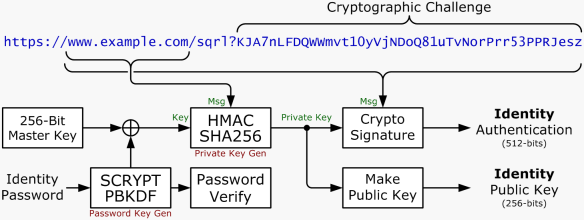
\includegraphics[width=.6\textwidth]{sqrl-arch.png}
	\caption{An Overview of SQRL's Crypto Architecture}
\end{figure}

\title{\textbf{The Cryptography of SQRL}}

As shown in the overview, both the Signature and Key functions start at the same 256-bit Master Key. This key is a static 256-bit random number that is either generated by the client, or imported from another device. In order for the system to be useful to both client and User the Master Key cannot change, so in order to maintain the security of the system the Master Key is encrypted by with a password using the Scrypt implementation of Password-Based Key Derivation Function. The process for deriving the Key from the User's password using this method is dependent upon the speed of memory to generate the key to help protect against brute-force password attacks, and to verify that the key is correct before moving on the next step, the Scrypt output key is processed one more time and the lower 128-bits are compared with the same lower bits that were generated when the password was initialized. Once the Scrypt key has been generated and verified, it is XORed with the Master Key to decrypt it for use in the next stage.

With the Master Key decrypted, the SQRL client takes it and the domain of the Host and passes them through the SHA256 hashing function. This is the private key that will be used to sign the 64-bit Cryptographic Challenge in order to prove User authenticity against an identity known to the Host, or a new Public Key that will form the basis of a new identity. The key piece of cryptography that drives this system here is the Ed25519 elliptic curve as implemented by Dan Bernstein. This function when supplied with both the domain-hashed Private Key and the Cryptographic Challenge provides the authentication string that will be sent to the Host as the proof of identity, where the Ed25519 function supplied with only the Private Key will produce the Public Key that is sent to the Host as the User's new identity.

\pagebreak

\title{\textbf{The Sea Squirrel Project}} 

\begin{enumerate}
	\item[\textbf{Goals:}] By the end of this semester the Sea Squirrel application will be able to
	\begin{enumerate}
		\item Create a new Master Key and import an existing Key.
		\item Encrypt and decrypt a Master Key based on a User-supplied password.
		\item Securely store multiple User IDs, and recall the available IDs.
		\item Create new Public Keys based on domain strings passed via argument.
		\item Answer Cryptographic Challenges based on domain strings and Host nonces passed via argument.
		\item Run as a headless back-end SQRL Identity Manager on all major desktop platforms.
		\item (optional) Run as a gtk+ gui application for linux systems.
	\end{enumerate}
	
	\item[\textbf{Challenges:}] In order to finish the Sea Squirrel project on time a significant number of pieces need to be build, but since all cryptographic primitives (Scrypt, SHA256, Ed25519) are available as part of the Sodium crypto library, what remains is to tie the various functions together as outlined in the SQRL architecture. Additionally, there already exists a completed SQRL client implemented in amd64 Assembly with test suites and implementation notes. The following need to be built.
	\begin{enumerate}
		\item An entropy harvester used to generate random noise for Master ID creation and for salting the password hashes.
		\item A User ID manager that will generate Master Keys, password verification strings, and salts for each unique User ID.
		\item A function to pass the User's password through the Scrypt algorithm with the required memory footprint of 16Mb, as well as to verify the output key against the stored Master ID.
		\item A parser to read 'sqrl://'-headed urls the Host's domain and Cryptographic Challenge.
		\item Functions to generate challenge-response and Public Key strings.
		\item A main driver that will read flags and arguments, read and store IDs to a file, and call the required SQRL functions.
	\end{enumerate}
	
\end{enumerate}

\nocite{*}	% causes all the references in the bib file to be included

\bibliography{sample}

\end{document}
